

\documentclass{beamer}

\mode<presentation> {

\usetheme{Boadilla}

\setbeamertemplate{footline}[page number] % To replace the footer line in all slides with a simple slide count uncomment this line

\setbeamertemplate{navigation symbols}{} % To remove the navigation symbols from the bottom of all slides uncomment this line
}
\usepackage[utf8]{inputenc}
\usepackage[brazil]{babel}
\setbeamercolor{alerted text}{fg=blue}
\usepackage{subfig}
\usepackage{graphicx} % Allows including images
\usepackage{booktabs} % Allows the use of \toprule, \midrule and \bottomrule in tables

%----------------------------------------------------------------------------------------
%	TITLE PAGE
%----------------------------------------------------------------------------------------

\title[ ]{\textbf{Modelo de otimização mutiobjetivo para adequação de embarcações de alta velocidade}\\Apresentação Parcial PAIC 2017/2018} % The short title appears at the bottom of every slide, the full title is only on the title page

\author[L.E.F.B]{Luiz Eduardo Fernandes Bentes, Renata da Encarnação Onety} % Your name
\institute[UEA] % Your institution as it will appear on the bottom of every slide, may be shorthand to save space
{
Universidade do Estado do Amazonas \\ Escola Superior de Tecnologia -- EST\\ Manaus - Amazonas - Brasil\\ % Your institution for the title page
\medskip
\textit{\{lefb.eng,ronety\} @uea.edu.br} % Your email address
}
\date{\today} % Date, can be changed to a custom date

\begin{document}

\begin{frame}
\titlepage % Print the title page as the first slide
\end{frame}

\begin{frame}
\frametitle{Overview}
\tableofcontents
\end{frame}

%------------------------------------------------
\section{Introdução} 
%------------------------------------------------
\begin{frame}
 \tableofcontents[ 
    currentsubsection, 
    hideothersubsections, 
    sectionstyle=show/shaded
    ] 
\end{frame}
%-------------------------------------------------
\begin{frame}
\frametitle{Introdução}
\begin{itemize}
	\item Para prestar socorro à população em atendimentos de urgência e emergência em saúde, as regiões sem acesso terrestre contam com o serviço de SAMU Fluvial.
	\item Atendimento similar às ambulâncias terrestres.
\end{itemize}

\begin{figure}[h]
	\centering
	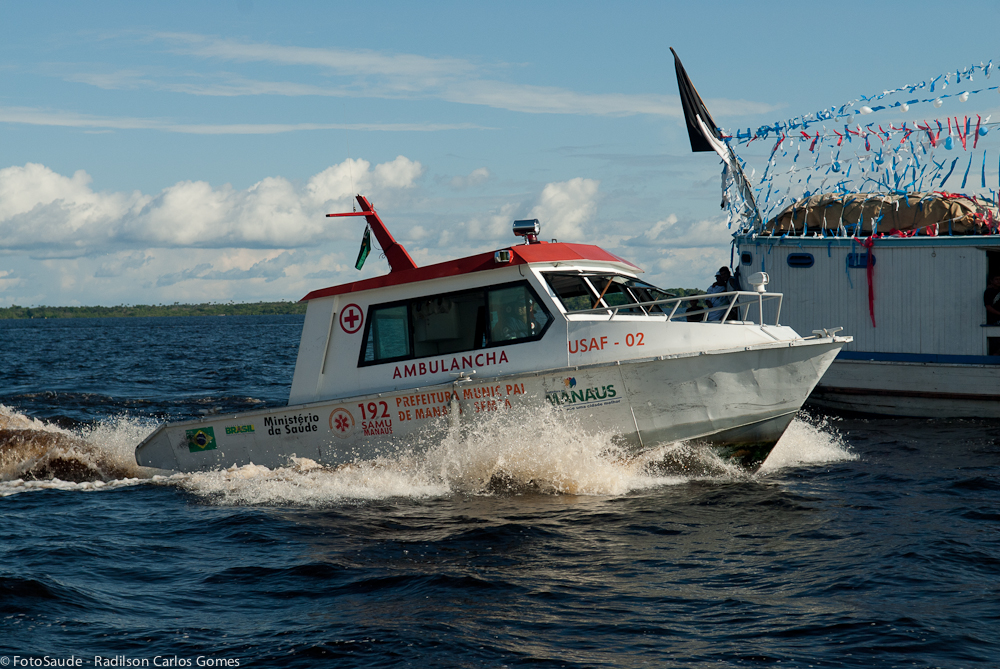
\includegraphics[scale=0.7]{samu17}
	\caption{Ambulâncias Fluviais}
	\label{fig:ambulancha}
\end{figure}

\end{frame}

%------------------------------------------------
\section{Justificativa}
%------------------------------------------------
\begin{frame}
\tableofcontents[ 
    currentsubsection, 
    hideothersubsections, 
    sectionstyle=show/shaded
    ] 
\end{frame}
%-------------------------------------------------
\begin{frame}
\frametitle{Justificativa}
\begin{itemize}
\item Atributos em relação à integridade estrutural devem ser atendidos
\item Modelo atual representa um projeto desenvolvido para meios marítimos.
\item Propor modelo que possa atender a população da melhor maneira possível  
\end{itemize}
\end{frame}
%-------------------------------------------------

\begin{frame}
\frametitle{Justificativa}
\begin{itemize}
	\item \alert{Atributos em relação à integridade estrutural devem ser atendidos}
	\begin{itemize}
		\item Estrutura suporte as cargas
		\item Ergonomia e bem-estar da tripulação
	\end{itemize}
	\item Modelo atual representa um projeto desenvolvido para meios marítimos.
	\item Propor modelo que possa atender a população da melhor maneira possível  
\end{itemize}
\end{frame}

%-------------------------------------------------
\begin{frame}
\frametitle{Justificativa}
\begin{itemize}
	\item Atributos em relação à integridade estrutural devem ser atendidos
	\item \alert{Modelo atual representa um projeto desenvolvido para meios marítimos}
	\item Propor modelo que possa atender a população da melhor maneira possível  
\end{itemize}
\end{frame}
%-------------------------------------------------
\begin{frame}
\frametitle{Justificativa}
\begin{itemize}
	\item Atributos em relação à integridade estrutural devem ser atendidos
	\item Modelo atual representa um projeto desenvolvido para meios marítimos
	\item \alert{Propor modelo que possa atender a população da melhor maneira possível}  
\end{itemize}
\end{frame}
%------------------------------------------------
\begin{frame}
\begin{figure}[h]
\centering
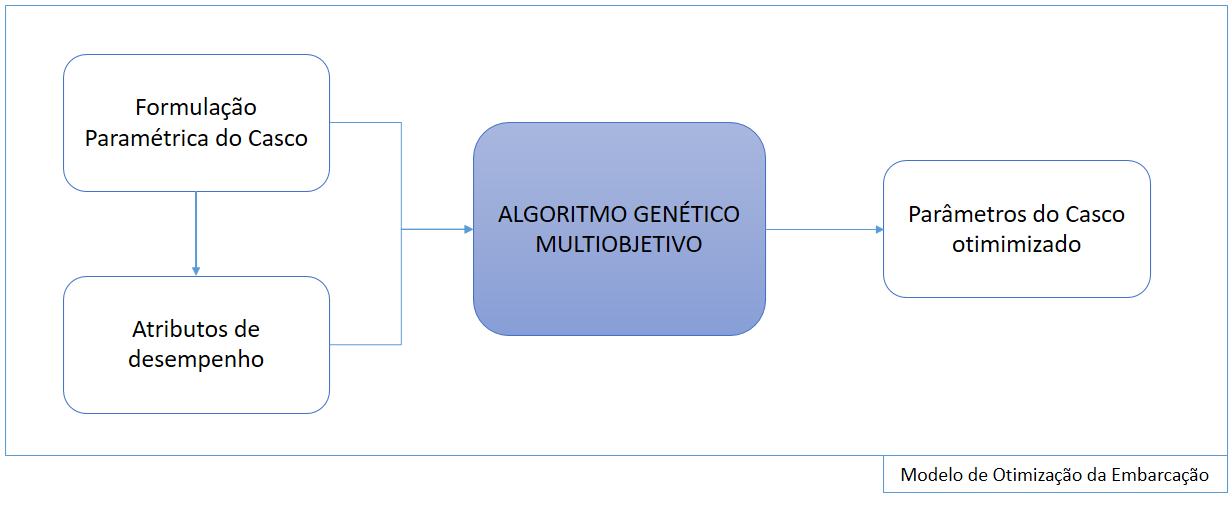
\includegraphics[scale=0.37]{img}
\caption{}
\label{fig:modelo}
\end{figure}
\end{frame}
%------------------------------------------------
\section{Objetivos}
%------------------------------------------------
\begin{frame}
\tableofcontents[ 
    currentsubsection, 
    hideothersubsections, 
    sectionstyle=show/shaded
    ] 
\end{frame}
%-------------------------------------------------
\begin{frame}
\frametitle{Objetivos}
\large
\begin{block}{Objetivo Geral}
Propor um modelo de otimização multiobjetivo baseado em Algoritmos Evolutivos para auxiliar no projeto de embarcações de alta velocidade, como as ambulanchas.
\end{block}
\pause
\begin{block}{Objetivos Específicos}
\begin{itemize}
\item Identificar métodos de construção de embarcações;
\item Desenhar o casco da embarcação através dos parâmetros de construção;
\item Propor algoritmo evolutivos para a otimização de variáveis do projeto
\item Implementar uma ferramenta computacional com interface amigável para auxiliar os projetistas desse tipo de embarcação.
\item Sugerir modelos de embarcações otimizadas.
\end{itemize}

\end{block}
\end{frame}
%-------------------------------------------------
\begin{frame}
\frametitle{Objetivos}
\large
\begin{block}{Objetivo Geral}
	Propor um modelo de otimização multiobjetivo baseado em Algoritmos Evolutivos para auxiliar no projeto de embarcações de alta velocidade, como as ambulanchas.
\end{block}
\begin{block}{Objetivos Específicos}
	\begin{itemize}
		\item \alert{Identificar métodos de construção de embarcações;}
		\item \alert{Desenhar o casco da embarcação através dos parâmetros de construção;}
		\item Propor algoritmo evolutivo para a otimização de variáveis do projeto
		\item Implementar uma ferramenta computacional com interface amigável para auxiliar os projetistas desse tipo de embarcação.
		\item Sugerir modelos de embarcações otimizadas.
	\end{itemize}
	
\end{block}
\end{frame}

%------------------------------------------------
\section{Fundamentação Teórica}
%------------------------------------------------
\begin{frame}
\tableofcontents[ 
    currentsubsection, 
    hideothersubsections, 
    sectionstyle=show/shaded
    ] 
\end{frame}
%-------------------------------------------------

\subsection{Curvas B-spline}
\begin{frame}{Curvas B-spline}
\begin{itemize}
\item Comumente usada na Engenharia Naval
\item Trata-se de uma curva formada por partes polinomiais
\item Polígono de Controle 
\end{itemize}

\begin{block}{Definição}
	\begin{equation}
		S(u) = \sum_{j = 0}^{n} {P_j B_j^n(u)} = \sum_{j = 0}^{n} {X_j B_j^n(u),Y_j B_j^n(u)}
	\end{equation}
\end{block}
\pause
\begin{figure}[h]
	\centering
	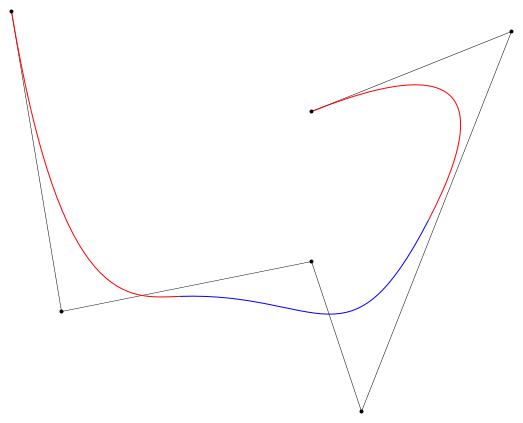
\includegraphics[scale=0.2]{bspline}
	\caption{Exemplo de Curva B-spline}
	\label{fig:bspline}
\end{figure}
\end{frame}

%------------------------------------------------

\subsection{Python + OpenGL}
\begin{frame}
\frametitle{Python + OpenGL}
\begin{itemize}
	\item OpenGL é uma API livre utilizada na computação gráfica
	\item GLUT - Interface para desenho das curvas. 
\end{itemize}

\begin{figure}[h]	
\centering

\includegraphics[width=4cm]{Python}
\qquad

\includegraphics[width=4cm]{logoopengl}
\end{figure}

\end{frame}    

%------------------------------------------------
\section{Resultados Parciais}
%------------------------------------------------
\begin{frame}
\tableofcontents[ 
    currentsubsection, 
    hideothersubsections, 
    sectionstyle=show/shaded
    ] 
\end{frame}
%-------------------------------------------------
\subsection{Vista Lateral}
\begin{frame}{Vista Lateral}
\begin{itemize}
	\item Formada por 3 curvas principais:
		\begin{itemize}
			\item Linha Central
			\item Linha \textit{Sheer}
			\item Linha \textit{Chine}
		\end{itemize}
	
\end{itemize}
\begin{figure}[h]
	\centering
	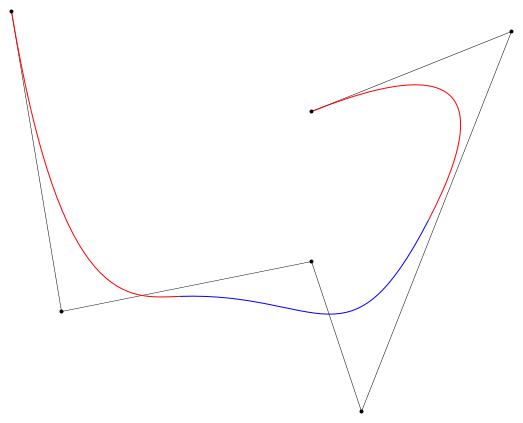
\includegraphics[scale=0.2]{bspline}
	\caption{Exemplo de Curva B-spline}
	\label{fig:central}
\end{figure}

\end{frame}
%-----------------------------------------------
\subsection{Vista Superior}
\begin{frame}{Vista Superior}
\end{frame}

%----------------------------------------------
\section{Trabalhos Futuros}
%----------------------------------------------
\begin{frame}
\tableofcontents[ 
    currentsubsection, 
    hideothersubsections, 
    sectionstyle=show/shaded
    ] 
\end{frame}
%-------------------------------------------------
\begin{frame}{Trabalhos Futuros}

\end{frame}

%----------------------------------------------
\section{Cronograma}
%---------------------------------------------
\begin{frame}{Cronograma}
\begin{table}[ht]
\centering

%\caption{My caption}
\label{my-label}
\begin{tabular}{|l|l|}
\hline
\multicolumn{1}{|c|}{Mês} & \multicolumn{1}{c|}{Atividades}                                                                                                                                                    \\ \hline
Março                     & \begin{tabular}[c]{@{}l@{}}Implementação do Algoritmo Genético\\ Desenvolvimento do Artigo para CSBC\\ Estudar Operadores Genéticos\end{tabular}                                   \\ \hline
Abril                     & \begin{tabular}[c]{@{}l@{}}Implementar novos Operadores\\ Desenvolver Componentes Híbridos\\ Implementação de novas restrições do problema geral \textit{Scheduling}\end{tabular} \\ \hline
Maio                      & \begin{tabular}[c]{@{}l@{}}Desenvolvimento do Artigo para SBPO\\ Execução de Testes com instâncias maiores\\ Teste das novas restrições\end{tabular}                               \\ \hline
Junho                     & \begin{tabular}[c]{@{}l@{}}Aperfeiçoar AG\\ Teste de novas instâncias\end{tabular}                                                                                                 \\ \hline
Julho                     & Apresentação Final                                                                                                                                                                 \\ \hline
\end{tabular}
\end{table}
\end{frame}

\section{Referencial Bibliográfico}
%----------------------------------------------
\begin{frame}{Referencial Bibliográfico}
  % estilo da bibliografia
  \bibliographystyle{abbrv}
  % chamando o arquivo refs.bib
  \bibliography{ref}
\end{frame}
% \subsection{Algoritmo Genético}
% \begin{frame}{Algoritmo Genético}

% \begin{itemize}
% \Large
% \item Método Heurístico
% \item Neo-Darwinismo (Evolução das Espécies)
% \item Componentes:
% \begin{itemize}
% \large
% \item Indivíduos
% \item População
% \end{itemize}
% \end{itemize}


% \end{frame}
%---------------------------------------------
% \begin{frame}{Funcionamento - Algoritmo Genético}
% \begin{figure}[h]
% \centering
% 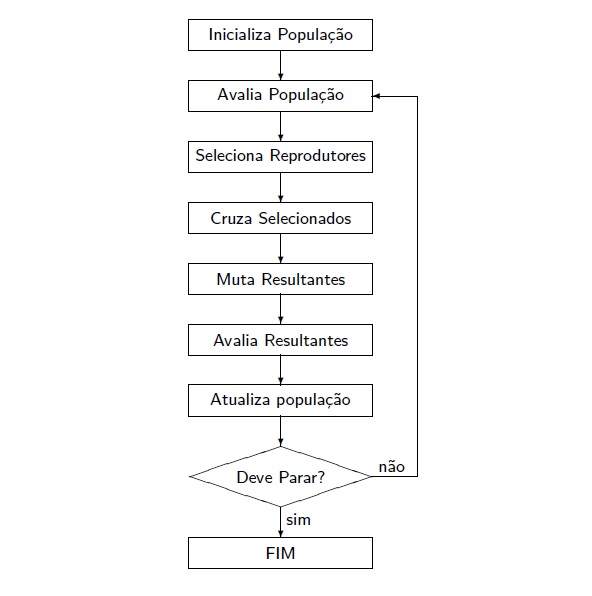
\includegraphics[scale=0.46]{Imagem7}
% \label{fig:funciomanentoAG}
% \caption{Funcionamento do Algoritmo Genético}
% \end{figure}
% \end{frame}
%---------------------------------------------
\begin{frame}
\titlepage
\end{frame}
%---------------------------------------------
\end{document}